\documentclass{article}
\usepackage{amsmath}
\usepackage{amsfonts}
\usepackage{amssymb}
\usepackage{enumitem}
\usepackage{tikz}

\title{MATH 222 - Assignment 1}
\date{January 2017}
\author{Daniel Frankcom}

\begin{document}
	\pagenumbering{gobble}
	\maketitle
	\setlength{\parindent}{0pt}
	\newcommand{\forceindent}{\leavevmode{\parindent=72pt\indent}}
	\newpage
	\pagenumbering{arabic}
	
	\begin{enumerate}
		\item We can solve this problem by using the fact that $\sum\limits_{v\in V}deg(v)=2|E|$
		\newline We know that $|E| = 29$
		\newline $\therefore 2|E|=58$
		\newline $\therefore\sum\limits_{v\in V}deg(v)=58$
		\newline Since each vertex must have at least degree 4, we can divide 58 by 4
		\newline $58\div 4=14.5$
		\newline $\therefore$ The maximum number of vertices that $G$ can have is 14, as the $.5$ can be accounted for by one or more vertices having slightly greater than a degree of 4
		
		\item If all vertices in $G$ have degree at least 2, then $G$ doesn't contain a cycle
		\newline However, if a graph does not contain a cycle, then there must be either a floating vertex, or a vertex with degree 1
		\newline $\therefore$ It is not possible for an acyclic graph to exist with all vertices having at least a degree of 2
		\newline $\therefore$ If all vertices in $G$ have degree at least 2, then $G$ contains a cycle
		
		\item Since a path of length 3 must contain 4 unique vertices, we can determine this number by choosing 4 of the 6 vertices in all possible combinations
		\newline This can be written as $\binom{6}{4}$
		\newline $\therefore$ The number of different subgraphs is $15$
		
		\item If $G$ is not connected, then there must be at least 2 distinct groups of connected components.
		\newline If group 1 has $n_{1}$ vertices, then any given vertex in this group may have a degree of $n_{1}-1$ at the most
		\newline If group 2 has $n_{2}$ vertices, then any given vertex in this group may have a degree of $n_{2}-1$ at the most
		\newline We know that $deg(x)+deg(y)\geq 19$
		\newline $\therefore n_{1}-1+n_{2}-1\geq 19$
		\newline $\therefore n_{1}+n_{2}-2 \geq 19$
		\newline $\therefore n-2 \geq 19$
		\newline $\therefore 20-2\geq19$
		\newline $\therefore 18\geq19$
		\newline $\therefore$ This case is not possible, and the only way that the conditions can be true, is if $G$ is connected
		
		\newpage
		\item Since there are 8 people and you received 7 answers back, we know that the numbers 0-6 must be present in the responses. We also know that there must be a duplicate, and that you must be one of the duplicates due to the fact that you received 7 different answers.
		\newline We know that the person who shook 0 hands must be partners with the person who shook 6 hands, since their partner shook every other person's hand. Using the same logic and working down recursively, we can figure out that 5 and 1 are partners, 4 and 2 are partners, and 3 and 3 are also partners.
		\newline Since we already knew that you were the duplicate, you and your friend both shook 3 hands.
		
		\item
		\begin{enumerate}
			\item Since a knight always moves from a white square to a black square and vice versa, the graph of possible moves can easily be seperated into 2 groups, with all of the black squares in one group, and all of the white squares in another.
			\item Each vertex has a different degree corresponding to the number of moves that a knight can make from each square. The potential moves for each square are detailed in the table below, with each square corresponding to a vertex in the graph.
			\newline 
			\begin{center}
				\begin{tabular}{llllllll}
					\multicolumn{1}{c}{2} & 3 & 4 & 4 & 4 & 4 & 3 & 2 \\
					3                     & 4 & 6 & 6 & 6 & 6 & 4 & 3 \\
					4                     & 6 & 8 & 8 & 8 & 8 & 6 & 4 \\
					4                     & 6 & 8 & 8 & 8 & 8 & 6 & 4 \\
					4                     & 6 & 8 & 8 & 8 & 8 & 6 & 4 \\
					4                     & 6 & 8 & 8 & 8 & 8 & 6 & 4 \\
					3                     & 4 & 6 & 6 & 6 & 6 & 4 & 3 \\
					2                     & 3 & 4 & 4 & 4 & 4 & 3 & 2
				\end{tabular}
			\end{center}
		\end{enumerate}
		
		\item
		\begin{enumerate}
			\item If a graph contains more than 4 vertices, then in one of the two partitions there must be at least 3 vertices. If this is the case, then the group of 3 or more vertices will not be incident to each other, following the definition of bipartite. This means that the complement will have these vertices connected in every way possible, certainly resulting in a cycle. This is contrary to the definition of bipartite, therefore it is not possible to partition a graph with 5 vertices such that both the graph and its complement are bipartite.
			
			\newpage
			\item In order for a graph to be self-complementary, it must be isomorphic to its complement. In order for this to be true, each of the 2 graphs must contain exactly half of the possible edges.
			\newline $|E| = \sum\limits_{v\in V}deg(v)= \frac{n(n-1)}{2}$
			\newline $\therefore \frac{|E|}{2}=\frac{n(n-1)}{4}$
			\newline $\frac{|E|}{2}$ must be an integer, as we cannot have part of an edge in our graphs. This means that the numerator must be divisible by 4.
			\begin{enumerate}
				\item $\frac{n(n-1)}{4}, n=4k$
				\newline $\frac{(4k)(4k-1)}{4}$
				\newline $k(4k-1)$
				
				\item $\frac{n(n-1)}{4}, n=4k+1$
				\newline $\frac{(4k+1)(4k+1-1)}{4}$
				\newline $\frac{(4k+1)(4k)}{4}$
				\newline $k(4k+1)$
			\end{enumerate}
			In both cases, the result is an integer, so if G is self-complementary, then $n=4k$ or $n=4k+1$.
		\end{enumerate}
		
		\item
		\begin{enumerate}
			\item If $K_{m,n}$ has a Hamiltonian cycle, then $m=n$ since the path must zigzag between each of the partitions and eventually reconnect with the starting node. If $m!=n$ then a vertex will need to be revisited (contrary to the definition of a Hamiltonian cycle), or the path will not be able to reconnect to the starting vertex (again contray to the definition).
			\newline Additionally, if $K_{m,n}$ has an Euler circuit, then $n$ must be even since in order for a graph to contain an Euler circuit it must have no more than 2 vertices with odd degree.
			
			\item The graph below contains an Euler circuit, but does not contain a Hamiltonian cycle.
			\newline
			\begin{center}
				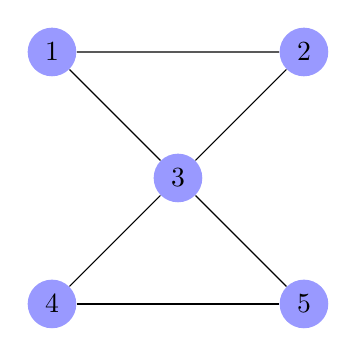
\begin{tikzpicture}
				[scale=.8,auto=left,every node/.style={circle,fill=blue!40}]
				\node (n5) at (5,1)  {5};
				\node (n4) at (1,1)  {4};
				\node (n3) at (3,3) {3};
				\node (n2) at (5,5)  {2};
				\node (n1) at (1,5)  {1};
				
				\foreach \from/\to in {n1/n2,n1/n3,n2/n3,n4/n3,n4/n5,n5/n3}
				\draw (\from) -- (\to);
				
				\end{tikzpicture}
			\end{center}
			$\therefore$ This statement is false
			
			\item The graph $K_{3,3}$ contains a Hamiltonian cycle, however does not contain an Euler circuit, as mentioned in part (a).
			\newline $\therefore$ This statement is false
			
			\item The 2 graphs both contain 5 vertices, 6 edges, and are nonisomorphic.
			\newline
			\begin{center}
				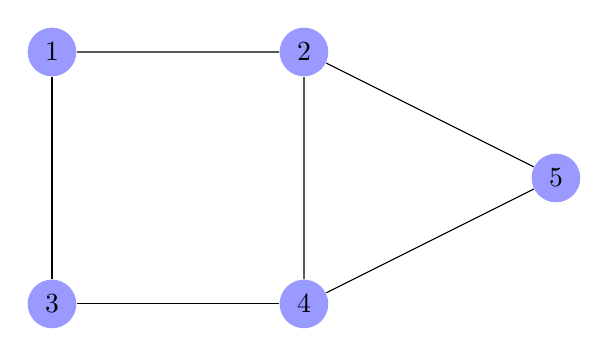
\begin{tikzpicture}
				[scale=.8,auto=left,every node/.style={circle,fill=blue!40}]
				\node (n5) at (12,6)  {5};
				\node (n4) at (8,4)  {4};
				\node (n3) at (4,4) {3};
				\node (n2) at (8,8)  {2};
				\node (n1) at (4,8)  {1};
				
				\foreach \from/\to in {n1/n3,n1/n2,n3/n4,n2/n4,n2/n5,n4/n5}
				\draw (\from) -- (\to);
				\end{tikzpicture}
				
				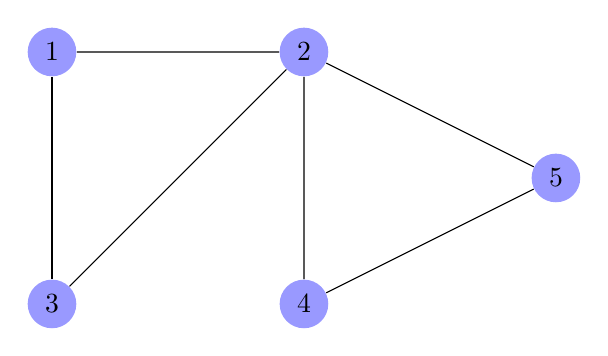
\begin{tikzpicture}
				[scale=.8,auto=left,every node/.style={circle,fill=blue!40}]
				\node (n5) at (12,6)  {5};
				\node (n4) at (8,4)  {4};
				\node (n3) at (4,4) {3};
				\node (n2) at (8,8)  {2};
				\node (n1) at (4,8)  {1};
				
				\foreach \from/\to in {n1/n3,n1/n2,n3/n2,n2/n4,n2/n5,n4/n5}
				\draw (\from) -- (\to);
				\end{tikzpicture}
			\end{center}
			$\therefore$ This statement is true
		\end{enumerate}
	\end{enumerate}
\end{document}